\section{PCB \& Enclosure}

	\subsection{PCB}	
	
		\begin{figure}[ht!]
			\centering
			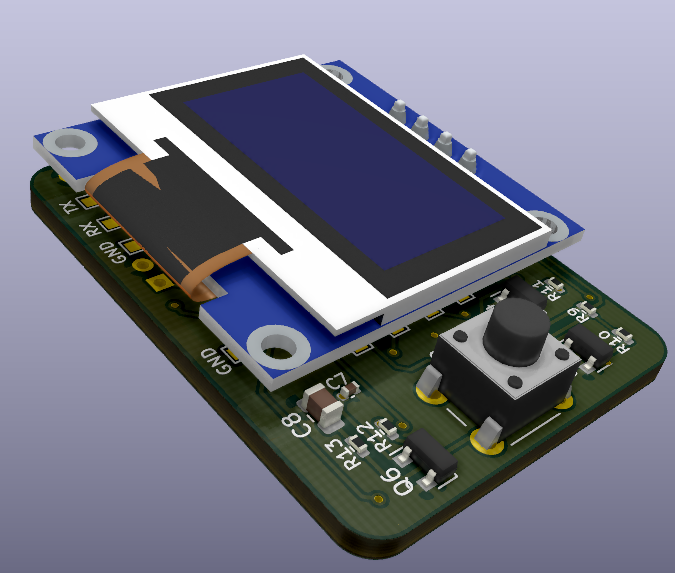
\includegraphics[width=0.6\textwidth]{../common/pcb/pcb.png}
			\caption{Completed PCB}
		\end{figure}


		\begin{figure}[ht!]
			\centering
			\subfloat[PCB Back
			]{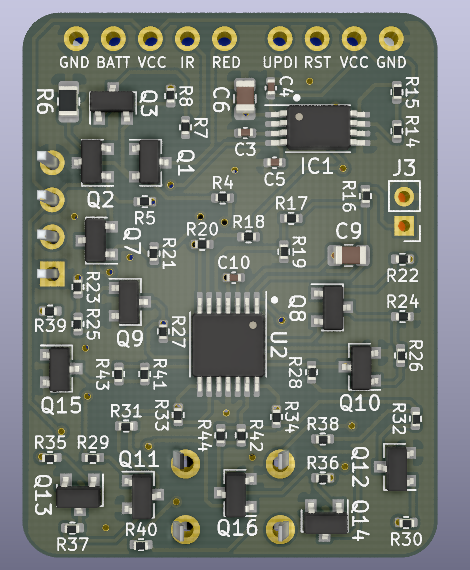
\includegraphics[width=0.5\textwidth]{../common/pcb/pcb_back.png}}
			\hfill
			\subfloat[PCB Front
			]{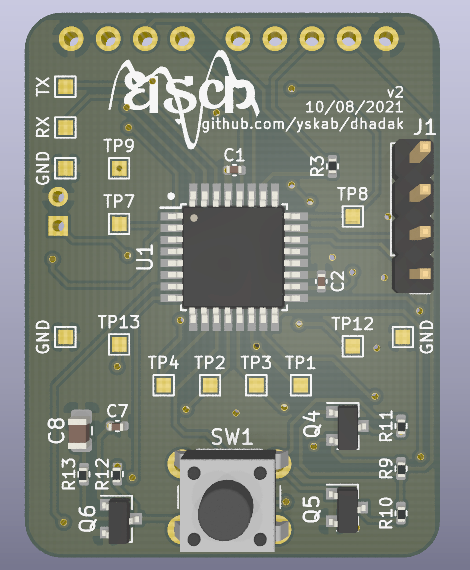
\includegraphics[width=0.5\textwidth]{../common/pcb/pcb_front.png}}
			\caption{PCB Images}
		\end{figure}

		PCB Design was completed on 2 layers with most of the components placed on the back side so that they can be re-flowed easily on a dosa pan. All components on front side are to be hand soldered.
		
		\begin{itemize}
			
			\item Design also includes a soft latch power on/off switch circuit to easily operate the device.
			
			\item A programming header was also added to program the $\mu$C via UPDI interface.
			
			\item Connection headers were added to connect the leds, battery \& photodiode which will be present on bottom compartment of enclosure.
			
			\item Header to attach OLED Display.

		\end{itemize}
	
		Sufficient test points were added on front side for easy access to probe and view the signals on oscilloscope.
		
		To keep the PCB size equivalent to that of the OLED display module, 0402 size resistors/capacitors were used.
			

	\subsection{Enclosure}		
		
		Enclosure was designed taking reference from a typical Oximeter which has display \& PCB on top, a finger insert below and a bottom part with battery compartment.
		
		\begin{figure}[ht!]
			\centering
			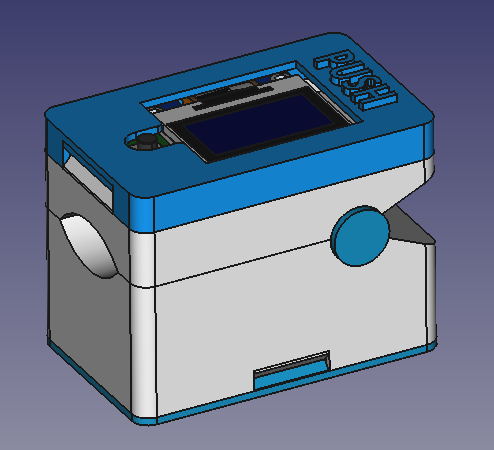
\includegraphics[width=0.5\textwidth]{../common/enc/enc.png}
			\caption{Completed Enclosure}
		\end{figure}	
		
				
		A reflective setup was implemented with photodiode on top base and pulse leds in bottom compartment. 
				
		\begin{figure}[ht!]
			\centering
			\subfloat[Photodiode compartment
			]{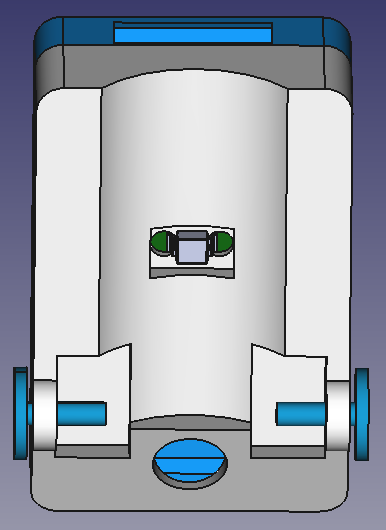
\includegraphics[width=0.45\textwidth]{../common/enc/top_base.png}}
			\hfill
			\subfloat[Spacers for pcb
			]{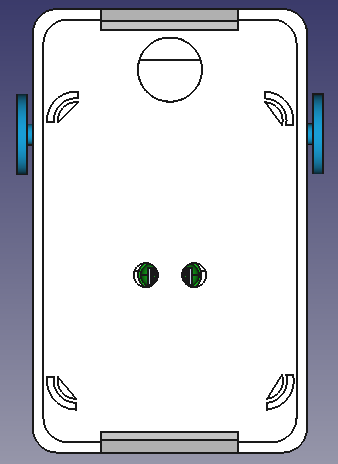
\includegraphics[width=0.45\textwidth]{../common/enc/top_base2.png}}
			\caption{Top Base}
		\end{figure}
	
	
		\begin{figure}[ht!]
			\centering
			\subfloat[Battery compartment
			]{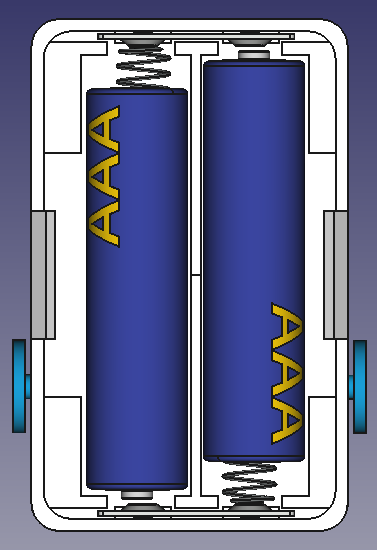
\includegraphics[width=0.45\textwidth]{../common/enc/bot_base.png}}
			\hfill
			\subfloat[Led compartment
			]{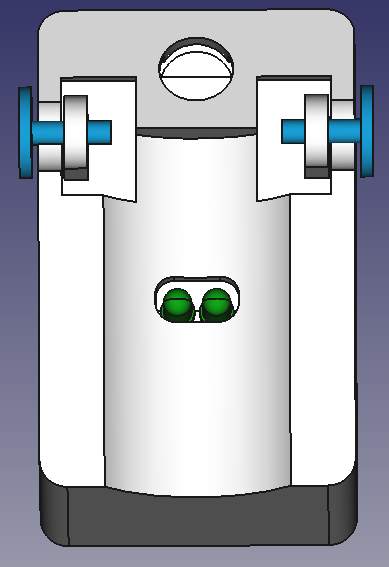
\includegraphics[width=0.45\textwidth]{../common/enc/bot_base2.png}}
			\caption{Bottom Base}
		\end{figure}
	
	
		Securing finger is an important part as any wobble or improper contact would lead to degradation in signal quality and calculated parameters. To achieve a firm pressure onto the finger which would hold it stable in place, a safety pin was used (removing the clip part) in the rotation mechanism.
		
		\begin{figure}[ht!]
			\centering
			\subfloat[Safety pin
			]{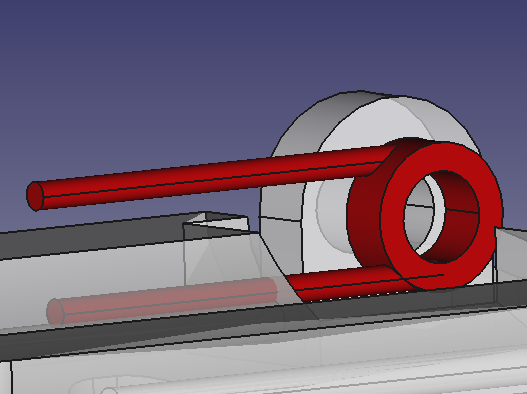
\includegraphics[width=0.5\textwidth]{../common/enc/pin.png}}
			\hfill
			\subfloat[Side view of pin
			]{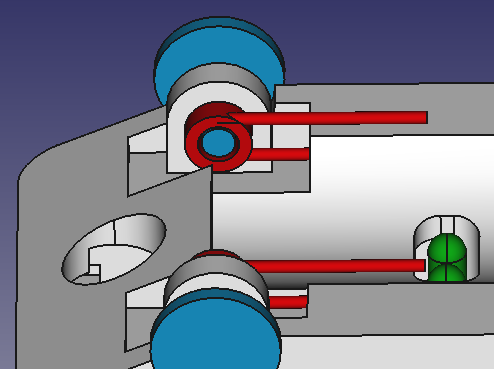
\includegraphics[width=0.5\textwidth]{../common/enc/pin_side.png}}
			\caption{Pin mounted in bottom base}
		\end{figure}	
		
		In idle position, pin would be in natural non-extended state hence both base parts would be closed. When a finger is inserted, lid needs to go up via the rotational mechanism as that is the only path to accommodate the finger. This would cause the upper part connected with pin to push down on finger which would lead to a firm grip to form ensuring good contact with photodiode and led.

		\begin{figure}[ht!]
			\centering
			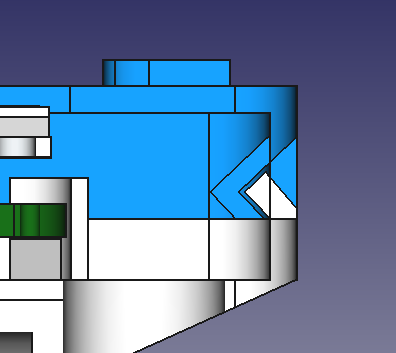
\includegraphics[width=0.6\textwidth]{../common/enc/snap.png}
			\caption{Snap fit cross-section}
		\end{figure}	
		
	
		Snap fit elements were implemented making it easier to fit and remove the cover parts whenever required.
